\documentclass{beamer}

\usepackage{graphicx}

\begin{document}

\begin{frame}{History}
    \begin{itemize}
        \item Need for a solution that can execute complex math required for DSP
        \item Originally, DSP applications implemented using bit-slice processors
        \item First DSP created by TI in 1978, used in Speak & Spell children's toy
        \item Second generation ~(80s) processors become standalone devices
        \item Third generation ~(90s) procesors allow hardware acceleration for complex math
        \item Fourth generation (current), higher clock speeds, smaller packaging, reduced price
    \end{itemize}
\end{frame}

\begin{frame}{Uses}
    \begin{itemize}
        \item Real-time data transformation % Cable box
        \item High performance data transformation % Audio/Video encoding
        \item Highly parallel computation % Bitcoin mining?
        \item Not for linear jobs % Can't take advantage of the parallelism
        \item Not for running a "modern" operating system % No virtual memory
    \end{itemize}
\end{frame}

\begin{frame}{What Is A DSP?}
    % TODO John
\end{frame}

\begin{frame}{Performance vs. Price}
    \begin{center}
        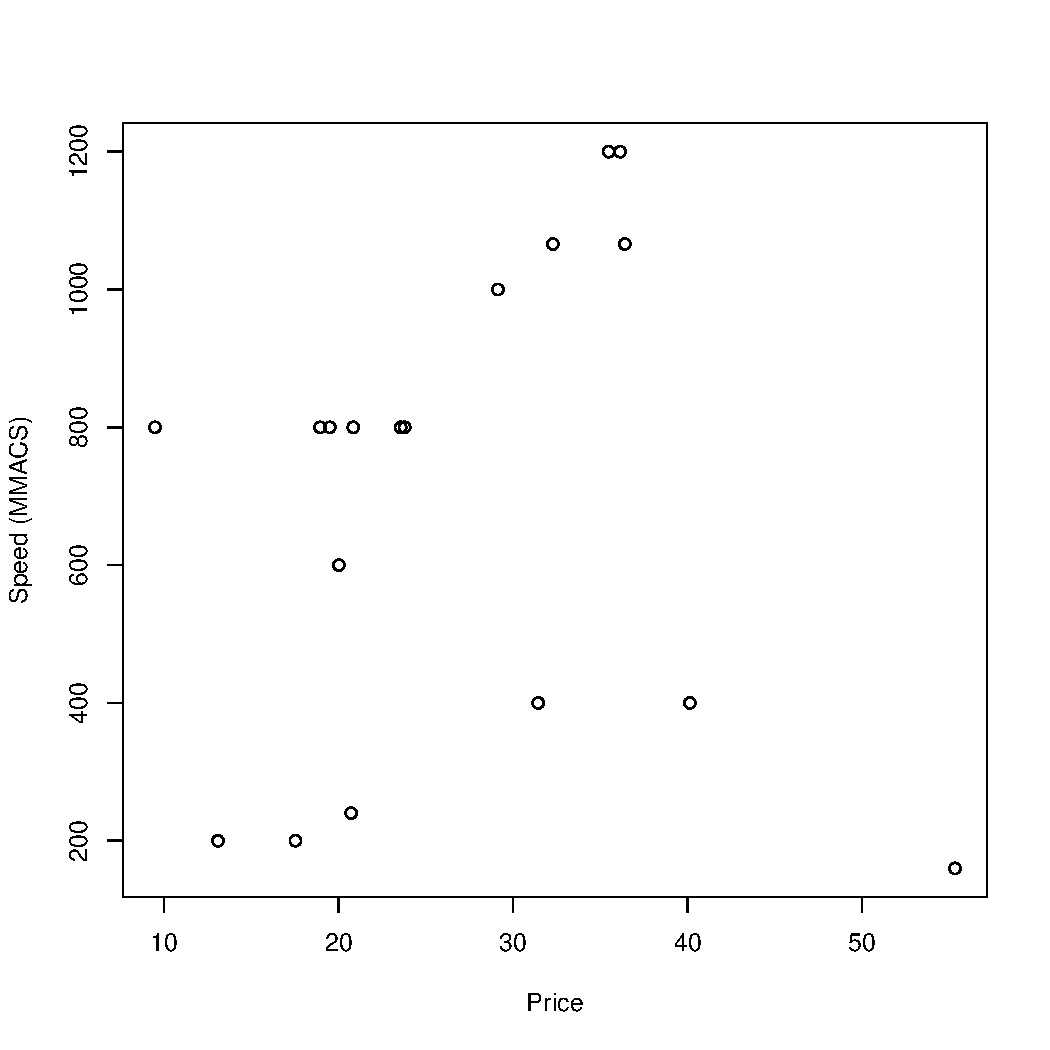
\includegraphics[width=0.8\textwidth]{price_perf.pdf}
    \end{center}
\end{frame}

\begin{frame}{Performance vs. Power}
    \begin{center}
        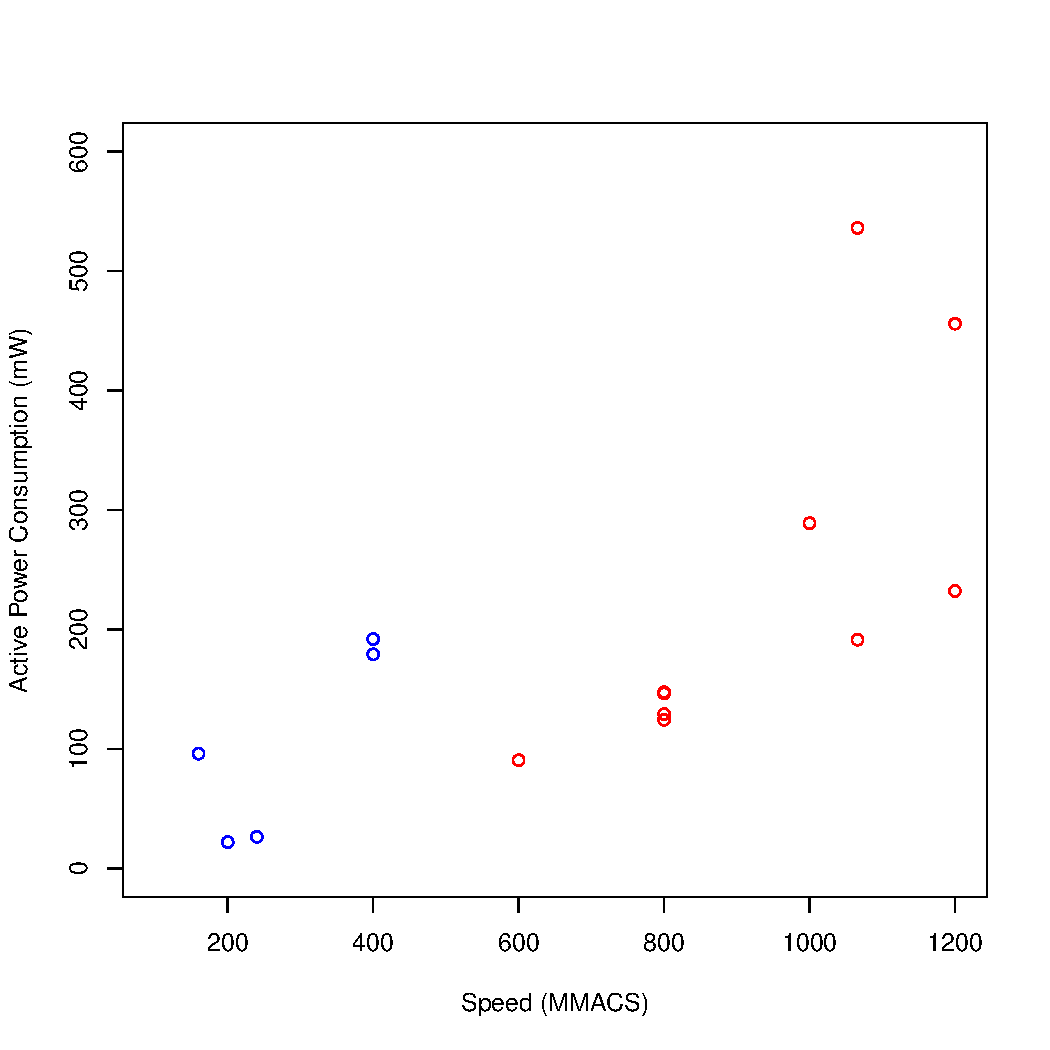
\includegraphics[width=0.8\textwidth]{power_perf.pdf}
    \end{center}
\end{frame}

\begin{frame}{How To Program a DSP}
    \begin{itemize}
        \item Architecture Description
            \begin{itemize}
                \item All available memory
                \item Memory mapped to external peripherals
            \end{itemize}
        \item Source Code Generation
            \begin{itemize}
                \item Slow but easy: High level languages such as C
                \item Fast but difficult: processor's native assembly
                \item Compromise: High level for generic functions, assembly for DSP computations
            \end{itemize}
    \end{itemize}
\end{frame}

\begin{frame}{FIR Filter in C}
    %snapshot of code
\end{frame}

\begin{frame}{FIR Filter in Assembly}
    %snapshot of code
\end{frame}

\begin{frame}{FIR in Assembly in a C program}
    %snapshot of code
\end{frame}

\begin{frame}{ISA}
    % TODO Alec
    \begin{itemize}
        \item Special instruction: MAC
    \end{itemize}
\end{frame}

\end{document}
